\documentclass[11pt,a4paper]{article}
\usepackage[utf8]{inputenc}
\usepackage[english]{babel}
\usepackage{amsmath}
\usepackage{amsfonts}
\usepackage{amssymb}
\usepackage{graphicx, wrapfig}
\usepackage[left=2cm,right=2cm,top=2cm,bottom=2cm]{geometry}
\usepackage[hidelinks]{hyperref} 
\usepackage{url}
\usepackage{listings}
\usepackage{color}
\usepackage[inline]{enumitem}
\usepackage{multicol}
\usepackage{tcolorbox}
\usepackage[bottom]{footmisc}
\usepackage{caption}
\captionsetup{font={small,sf}} % For caption fonts
\captionsetup[sub]{font={small,sf}} % For caption fonts

\usepackage[maxnames=99,maxcitenames=2,style=authoryear]{biblatex}

\addbibresource{refs.bib}

\title{\textbf{Advanced Machine Learning (WS 2020/21) \\Programming Project}}
\date{}
\begin{document}
\maketitle
\vspace{-3em}

\begin{tcolorbox}[
size=tight,
colback=white,
boxrule=0.2mm,
left=3mm,right=3mm, top=3mm, bottom=1mm
]
{\begin{multicols}{3}

\textbf{Author 1}       \\
Last name: Gugglberger               \\  % Enter first name
First name: Josef            \\  % Enter first name
c-Number: csat2151               \\  % Enter c-number

\columnbreak

\textbf{Author 2}       \\
Last name: Kommer             \\  % Enter first name
First name: Phillip             \\  % Enter first name
c-Number: csat3364             \\  % Enter c-number

\columnbreak

\textbf{Author 3}       \\
Last name: Peintner               \\  % Enter first name
First name: Andreas             \\  % Enter first name
c-Number: csas7462               \\  % Enter c-number

\end{multicols}}
\end{tcolorbox}


\section{Introduction}
\label{sec:intro}
%Describe the problem you are solving (very briefly), and also include a short overview of your approach and how the rest of the report is organized. Point the reader to your main findings.

As part of the seminar in advanced machine learning a final programming project is conducted to get detailed insights on modern reinforcement learning algorithms. These algorithms are tested against the \textit{Acrobot-v1} environment, which is included in OpenAI Gym (\cite{openai-gym}). %TODO image?

To be more specific, the environment consists of a 2-link pendulum, with only the joint between the two links that can be controlled. The continuous state space of this environment comprises the two rotational joint angles and the joint angular velocities. Following discrete actions can be applied on joint: +1, 0 or -1 torque. 

Q-Learning with a neural network as the function approximator deals as a baseline model. Additionally, the modern deep reinforcement algorithms Deep Q Network (DQN) and the actor-critic based Advantage Actor Critic (A2C) are implemented and compared to each other in respect of performance and stability. % TODO cite here?

The rest of this report is structured as follows: in Section \ref{sec:methods} chosen reinforcement learning algorithms to tackle the task are described. Section \ref{sec:setup} presents our experimental setup and used hyperparameters. Results of the individual agents on the specified environment and comparisons of performance are shown in Section \ref{sec:exp}. Section \ref{sec:con} will wrap up the main findings and analyze the results of the conducted experiments.


\section{Methods}
\label{sec:methods}
%Mention the algorithms you have chosen, and describe the reasons for your choice. You don't have to describe the algorithms in detail. Remember to include relevant references.

Q-learning allows to find an optimal action-value function by using temporal difference updates. The agent will perform the sequence of actions that generate the maximum total reward (the Q-value). For large or infinite state space, where it is infeasible to store a table of all the states and actions, value function approximation is used, which allows to make use of deep neural networks as approximators. In value function approximation a value function is parameterized by some weight vector that is much smaller than the number of states. This weight vector then gets updated during training to enable the value-function to predict the true value of states. Q-learning with a neural network as the function approximator (Deep Q-learning) can be seen as a Deep Q Network without any extensions.\\

The second algorithm we implemented was a Deep Q Network (DQN). \cite{mnih2013playing} proposed the first reinforcement learning algorithm using deep neural networks. The authors showed that agents can learn a value function directly from raw input pixels of Atari games. Convolutional Neural Networks (CNNs) were trained with Q-learning and a technique called experience replay, a concept first introduced by \cite{lin1992self} . In each step, a tuple containing state, action, reward, and the next state is appended to a queue. The Q-learning update is then performed on a batch of tuples sampled randomly from the queue. According to \cite{sutton2018reinforcement}, this has following advantages: first, every experience is used (potentially) more than once, which can reduce the required number of episodes. Secondly, consecutive samples have a high correlation with each other. Due to the random sample, samples inside batches are not correlated with each other, resulting in a higher variance and therefore a stabler training. 

Because DQN results were unstable in our first experiments, we decided to implement an extension known as Double DQN (DDQN), proposed by \cite{van2016deep}. The idea is to use two deep neural networks, one for action-selection, and the other one for action-evaluation. Using one network for the two tasks results in overestimating values. In Double DQN one network is updated in each time step, and the other network is used just for evaluation (the target network). The target network is then updated by copying the weights every $N$ time step, where $N$ is a fixed number (usually around $100$).

It should be noted here that \cite{mnih2013playing} defined DQNs as Q-learning that uses deep convolutional networks. However, the \textit{Acrobot-v1} environment does not expose pixel values of the environment, but rather position and velocity of joints. Therefore it does not make sense to use a CNN, instead we used a (deep) dense network. \\

The last algorithm we chose is Advantage Actor Critic (A2C). As one can recognize from the name, this is a progression to the "normal" Actor Critic algorithm. Here two networks are used, the Actor and the Critic. The Critic estimates the value function. The Actor makes the steps and uses the suggestions from the Critic to update the policy distribution. This combination of acting and criticizing should in theory merge the advantages of both value-based and policy-based algorithms.

The "Advantage" in A2C comes from a change in the critic. In A2C the critic uses the Advantage-value \textit{A(s,a)} instead of the Q-value. This way the agent can determine how much better an action can be. Using the advantage function reduces the high variance of policy networks and stabilize the model (\cite{actorCritics}).\\ 


\section{Setup}
\label{sec:setup}
% Describe your experimental setup. Clearly mention what hyperparameters you use for training your chosen algorithms. You can also describe here the structure of the neural networks that you use. Feel free to include any other setup-related information.
This section describes the experimental configurations that were used to train the different agents. Table \ref{tab:comparison_hyper} shows a comparison of the most important hyperparameters used for training.

Agents are optimized for the OpenAI Gym environment \textit{Acrobot-v1}. The reward for swinging the pendulum above the line in the environment is $0$, while the agents get a reward of $-1$ for every timestep it fails to do so.

\subsection{Deep Q-Learning}

The deep Q-learning agent is heavily based on the code given by Sayantan Auddy (available on OLAT) and uses PyTorch as deep learning library. Since this method is quite simple, it can struggle with the maximal step size of this environment (500). So the maximal step size of the environment is set to 4000 for the deep Q-learning agent. The simplicity of the Q-learning agent lead to the choice of a low number of episodes and a high number of steps per episode for training to get stable results as can be seen in Table \ref{tab:comparison_hyper}. The two layers of the value approximator network have 200 hidden units each and are combined via the ReLU activiation function. Adam is used for optimization and the mean squared error as loss function. The learning rate is 0.0001, $\gamma$ is 0.99 and the exploration rate of the agent is set to 0.3. We trained the agent 5 times and took the best result for evaluation.

\subsection{DQN \& DDQN}

The DQN and DDQN Agents were implemented using the deep learning libraries Keras and Tensorflow.

Both Agents, DQN and DDQN, were trained on the same set of parameters. The discount factor $\gamma$ is $0.95$, the exploration rate $\epsilon$ starts with $1.0$ and decays by multiplying with the factor $0.995$ every time the network weights are updated, while its minimal value is $0.01$. The learning rate is $0.001$, and the length of the queue used for the replay buffer is $10000$. The two dense layer of the neural network have $128$ hidden units, and it is trained in batches of size $128$. For performance reasons, the update interval is $8$, meaning that the network weights are not updated in every step, but in each $8^{th}$ step.

DDQN keeps a copy of the exact same network, called the target network. Its weights are updated every time $100^{th}$ time the other network is updated.

\subsection{A2C}
The A2C agent is implemented using PyTorch and can be executed via the jupyter notebook in the A2C folder. As mentioned in the "Methods" section the agent uses a two-headed network (the actor and the critic network). In this implementation both networks are combined into one for easier handling for the agent.

The agent starts out with random actions, where each action has the same probabilities. It continues to take random actions for the whole training, but with every episode the probability of each action gets adjusted according to the results from the last episode. Those adjustments are made based on two values, namely the actor loss (aka. policy loss) and the critic loss (aka. value loss). Those are then combined to one and with this value the network is updated. One thing to note here is that the critic loss is multiplied by 0.5 in order to give the actor loss more influence. This should result in a better training for the agent. There is also an entropy term to act as a penalty for actions with a significantly higher probability then the rest. This should prevent the agent from always taking the same action (\cite{actorCritics2}).


\subsection{Hyperparameters}

In order to keep the results comparable to each other, we chose the hyperparameters as similar as possible between all the algorithms. Still there are some differences between parameters, mostly to get better results for the given agent.\\

\begin{table}[h]
    \centering
    \begin{tabular}{|c|r|r|r|r|r|}
         Agent & episodes & steps & hidden units & learning rate & gamma\\
         \hline
         Q-learning & 200 & 2000 & 200,200 & 0.0001 & 0.99\\
         DQN & 1000 & 500 & 128,128 & 0.001 & 0.95\\
         DDQN & 1000 & 500 & 128,128 & 0.001 & 0.95\\
         A2C & 5000 & 500 & 128,128 & 0.0001 & 0.99\\
    \end{tabular}
    \caption{Comparison of hyperparamters used in agents.}
    \label{tab:comparison_hyper}
\end{table}


\section{Experiments and Results}
\label{sec:exp}
%Describe in detail how you trained your agents, and what the result of the training was. Compare the performance of your chosen algorithms against one another. As a lower baseline, also compare the performance of these algorithms against an agent that always takes random actions. Comment on the hyperparameters that you feel are important for performing well. You can also remark on specific features of your implemented algorithms that you feel contributed to their good or bad performance. All plots and tables should be included in this section (remember to use proper axis labels, legends, and titles for your plots).
The following section discusses the results obtained from training and checks how the different agents compare with each other. 

\subsection{Deep Q-Learning}
Experiments have shown that our implementation of deep Q-learning is highly sensitive to the chosen hyperparameters for training. Different configurations were applied to the agent, but none of them outperformed the original configuration given in the code example. Even small changes in the number of hidden untis or decreasing the number of steps lead to very unstable results. The original configuration stabilizes after about 100 episodes and reaches continuous rewards higher as 200. Training of the agent longer than 200 episodes also impacts the results negatively. Figure \ref{fig:qlearn_random_result} shows the deep Q-learning agent in comparison to a random agent. The random agent simply chooses random actions at every state and is not able to learn anything. It is surprising that the deep Q-learning agent delivers stable and competitive results in comparison to the other presented methods, although it needs less time for training and converges faster.

\begin{figure}[h]
\centering
\begin{subfigure}
    \centering
    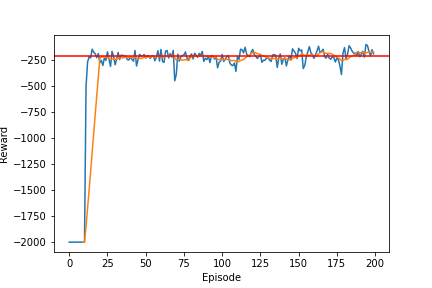
\includegraphics[width=0.48\linewidth]{images/qlearn.png}
\end{subfigure}%
\begin{subfigure}
    \centering
    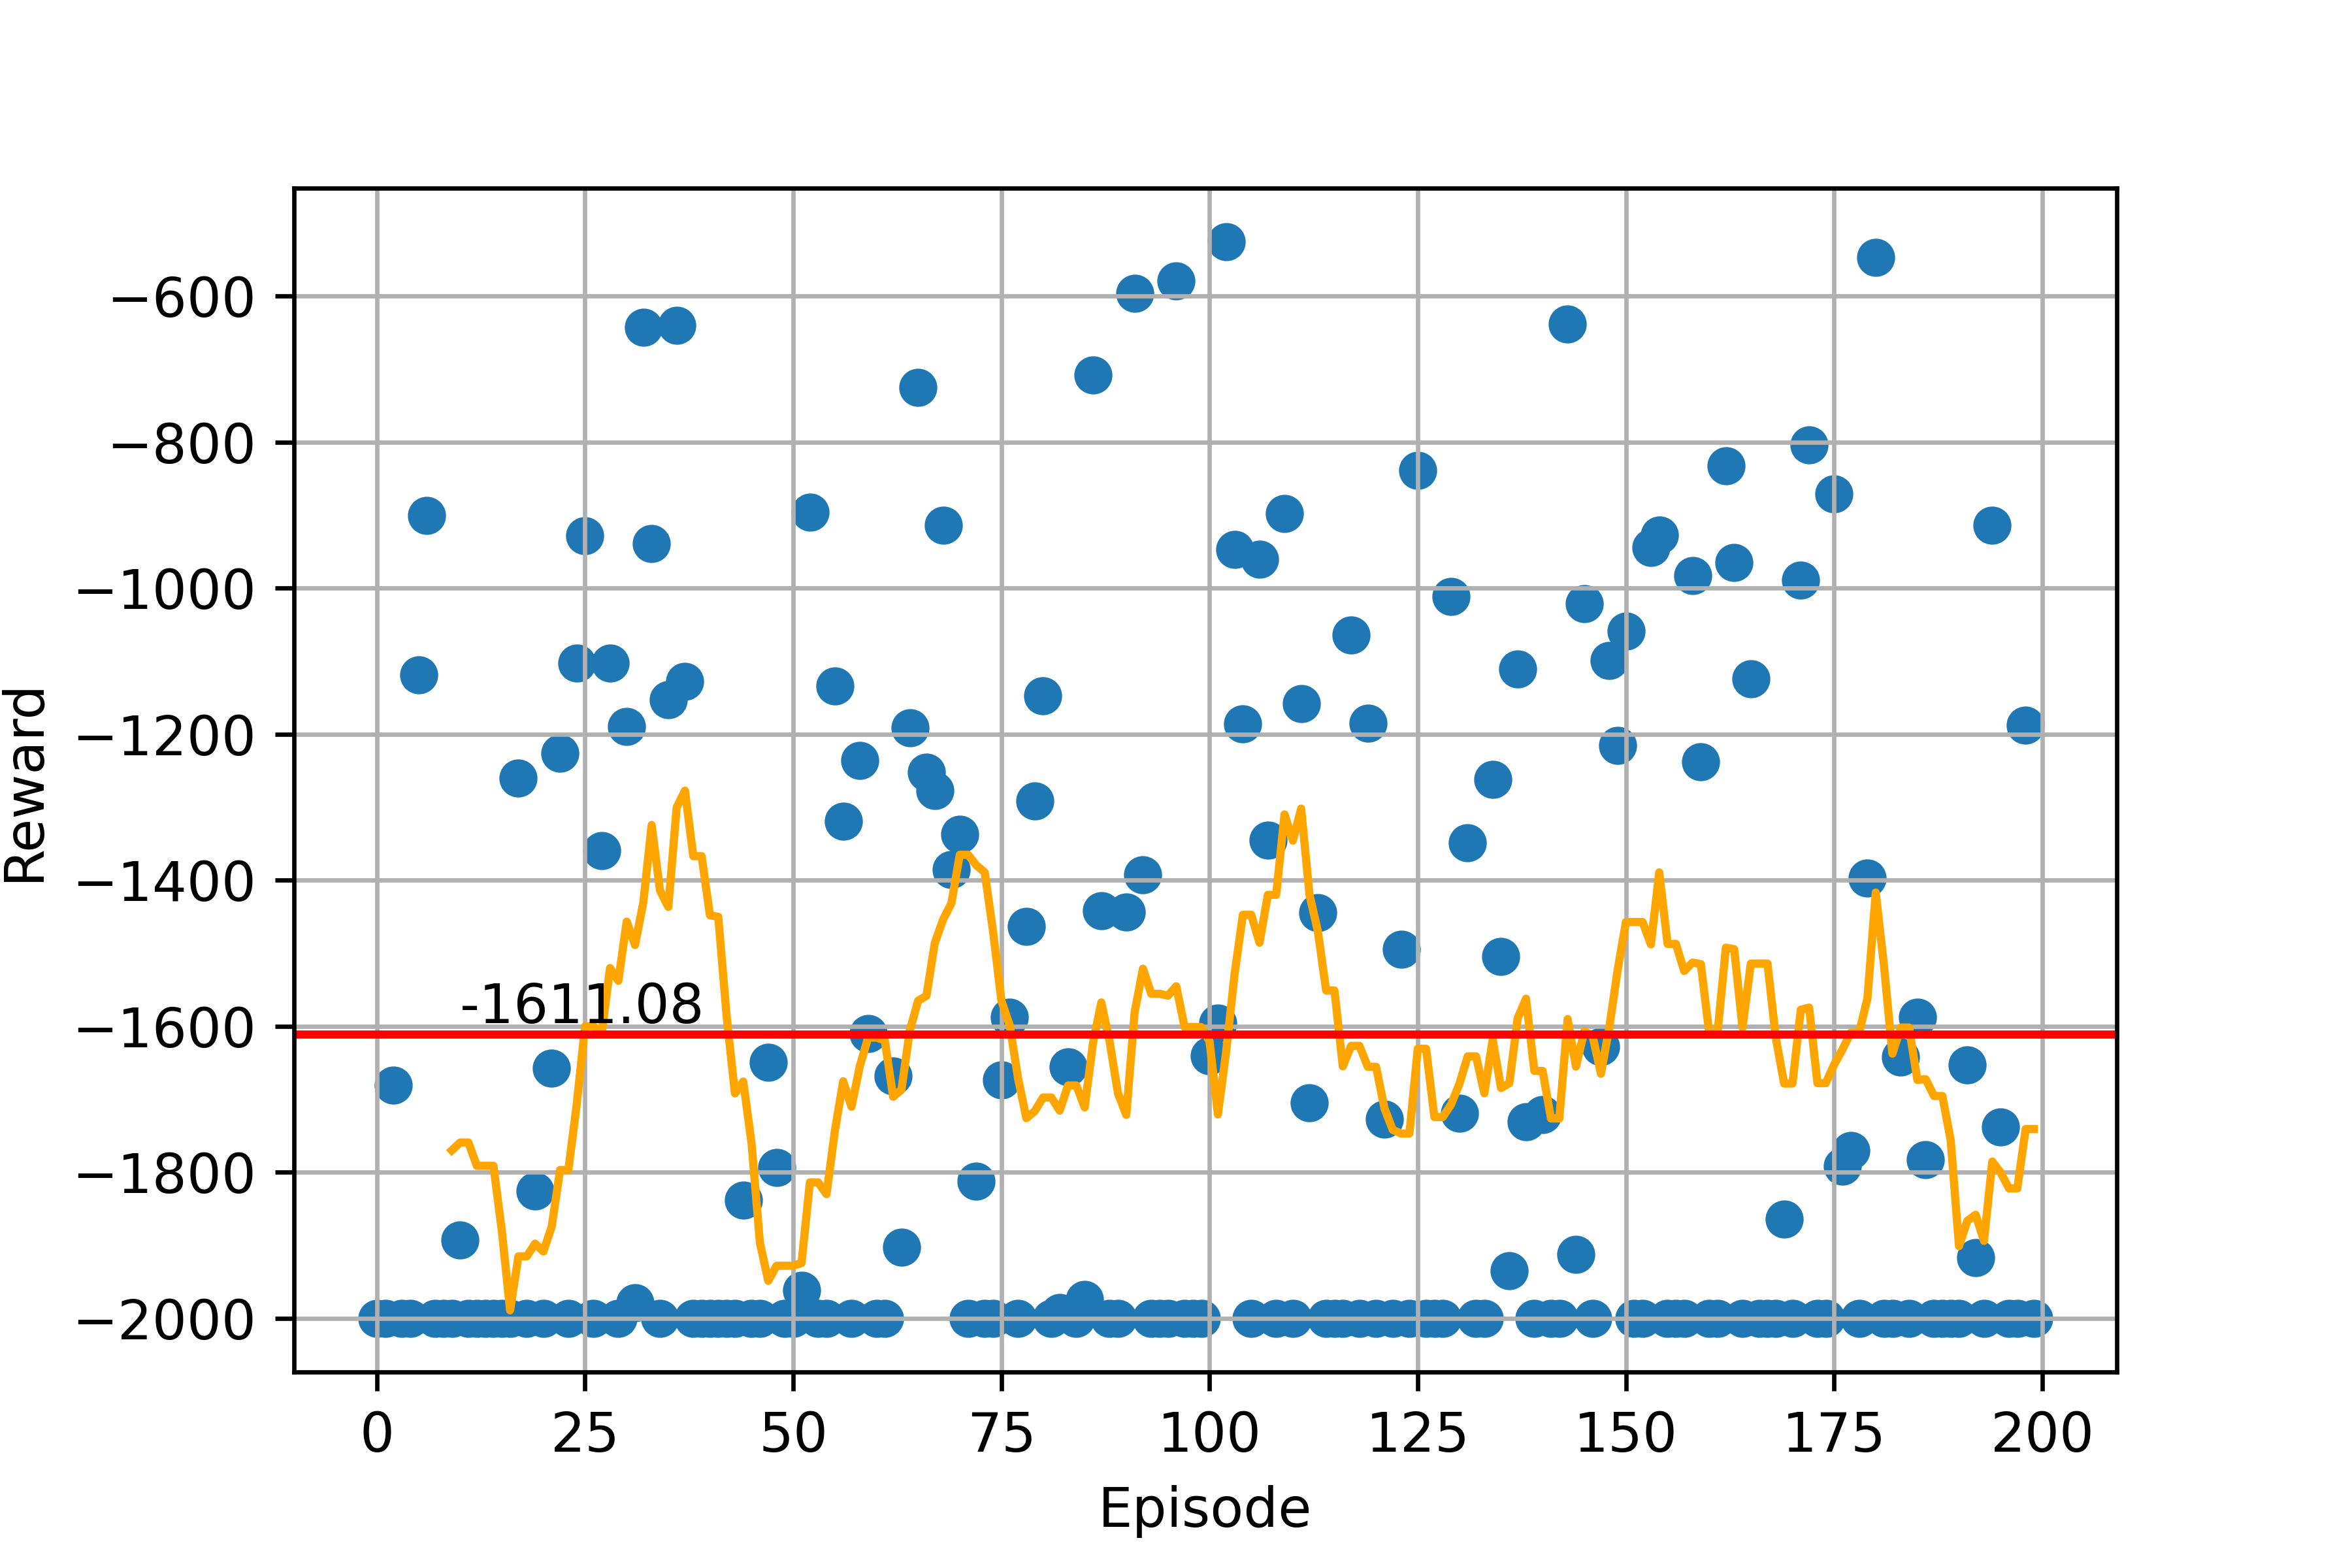
\includegraphics[width=0.48\linewidth]{images/random.png}
\end{subfigure}
\caption{This plot shows scores per episodes for Q-Learning Agent (left) and Random Agent (right) in the training process on Acrobot-v1. The red line shows the average score of the last 100 episodes and the orange line is an average of the last 10 episodes.}
\label{fig:qlearn_random_result}
\end{figure}

\subsection{DQN \& DDQN}

The DQN and DDQN agents were trained for $1000$ episodes with a maximum of $500$ steps. Details of the architecture and hyperparameters are discussed in Section \ref{sec:setup}.

Figure \ref{fig:dqn_ddqn_result} shows the scores per episode obtained in the training process for the DQN and the DDQN agent. The plot shows that the DQN agent was able to learn the task, but its performance is unstable. Even in the last $100$ steps there are some episodes which are rewarded by a score below $-300$. The average score of the last $100$ episodes is $-164.39$.
The DDQN agent not only performed better, it was also much more stable. There was no episode in the last $200$ steps that was rewarded below $-300$. Also the performance of the last $100$ episodes was, with an average score of $135.99$, much better than the performance of the DQN.

We started to train the DQN agent with two hidden layers with $64$ units. With this configuration the agent was able to master simpler environments like \textit{Cartpole-v1}, but it was not able to solve \textit{Acrobot-v1}. After increasing the number of units to $80$, which was also not enough, we arrived at using $128$ units. Unfortunately, we were not able to do a more comprehensive grid search for finding the best parameters, because training took a very long time (\sim$48h$).

\begin{figure}[h]
\centering
\begin{subfigure}
    \centering
    \includegraphics[width=0.48\linewidth]{images/dqn.png}
\end{subfigure}%
\begin{subfigure}
    \centering
    \includegraphics[width=0.48\linewidth]{images/ddqn.png}
\end{subfigure}
\caption{This plot shows scores per episodes for DQN (left) and DDQN (right) agent in the training process on Acrobot-v1. The red line shows the average score of the last 100 episodes and the orange line is an average of the last 10 episodes.}
\label{fig:dqn_ddqn_result}
\end{figure}



\subsection{A2C}

In contrast to the DQN agent, the training process for the A2C agent was a lot faster. Therefore we were able to train the agent for way more episodes, which was essential for this agent. To keep the results comparable, the maximum step size stayed at $500$, as for the other agents. 

The increase in episodes was needed because the A2C agent mostly starts out slow. Some training sessions took from $1000$ up to even $2000$ episodes before some progress was visible. This means that this agent is probably the least consistent of our agents, but as soon as some progress was made, the agent increases its performance at a solid rate. 

In effort to make the agent more consistent we tried changing some parameters, including increasing/decreasing the hidden units, but in the end the most effective optimization was to increase the number of episodes and let the agent train longer. In general the agent shows promising results after around $2000-3000$ episodes and flattens the curve at around $5000$, at which the agent converged in most of the training sessions.

As can be seen in \ref{fig:a2c_result} the average over the last $100$ episodes for this agent was $-181.31$. The orange line shows an average of the last 10 episodes to smooth the results. Unfortunately, there are still some episodes scoring really low even after $4000$ episodes, but all in all the agent is able to learn the task in a decent way.

\begin{figure}[h]
  \centering
  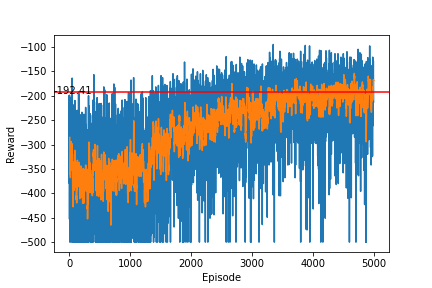
\includegraphics[scale=0.75]{images/a2c.png}
  \caption{This plot shows the results for the A2C agent. The red line shows the average score of the last 100 episodes and the orange line is an average of the last 10 episodes.}
  \label{fig:a2c_result}
\end{figure}

\subsection{Agent comparison}

As a metric for comparing our agents we decided to use the average scores obtained over the last 100 episodes of training. We also added the results of a random agent for comparison.

It is clear see in Table \ref{tab:score_comparison} that all implemented reinforcement learning approaches outperform the random agent by a lot. DDQN reached the highest average in rewards, followed by the DQN agent. The A2C method is not able to succeed the deep Q-learning agent, however training the agent a higher number of episodes could lead to better results, since it shows a trend towards higher rewards in the learning curve. 
We did some experiments in tuning the hyperparameters on all agents to increase there performance, but we are confident that there is still some potential for improvement for all of them. By doing an extensive grid search some hyperparameters could be tuned even further, but due to the lack of time, we had to omit such a procedure.

\begin{table}[h]
    \centering
    \begin{tabular}{|c|r|}
         Agent & Avg. score on last 100 episodes \\ 
         \hline
         Random &  -1534.59\\
         Deep Q-learning &  -179.36\\
         DQN & -164.39\\
         DDQN & \textbf{-135.99}\\
         A2C & -181.31\\
    \end{tabular}
    \caption{Comparison of different agents of the average score of the last 100 episodes.}
    \label{tab:score_comparison}
\end{table}

\section{Conclusion}
\label{sec:con}
% Analyze your results and summarize your main findings. Also, share your thoughts on how the performance of your algorithms can be improved further.

In this project we investigated several reinforcement learning approaches based on deep neural networks in detail. The highest score on the \textit{Acrobot-v1} environment is reached by the DDQN agent. Deep Q-learning shows the most stable results after 100 episodes, and the training procedure was significantly faster compared to the other agents. The A2C approach consistently improves the rewards over a high number of episodes and indicates possible improvements given better hardware and more time.

For future work, we propose following enhancements: 
\begin{enumerate*}
  \item The DQN and DDQN agents could be implemented with a \textit{prioritized} replay buffer, as proposed by \cite{schaul2015prioritized}. The key-idea of this approach is to replay more important transitions more often than other transition. The authors claim that this can speed up the learning process by a factor of $2$.
  \item Due to the long training times of the DQN and DDQN agent, we were not able to do a comprehensive grid search to find the best hyperparameters.
\end{enumerate*}

%\section{References}
\printbibliography


\end{document}